\section{Problem Set 5}

\subsection{What are the Control Objectives?}

\subsubsection{Significant Operational Modes}
The most significant operational modes of our mission will be station keeping, docking, and safety. As with all scientific missions, station keeping will occur when the spacecrafts are not required to do any observation or function, but rather hold position while other mission objectives are being accomplished, such as generating power or transmitting data. From a distributed space systems perspective, station keeping will require the spacecraft to maintain a stable configuration, sometimes in the vicinity of of the ISS. Therefore, it will be required to hold the same energy state and same semi major axis.

The next mode to consider is docking mode, where the dragon is moving itself closer to the ISS. This mode requires an inherent instability and difference in semi major axis, where an approach is being made purposefully.

Finally, the last mode is safety mode, which also includes a difference in semi major axis because the dragon should back away from the station in this scenario. It does not necessarily have to be fast, but rather, safety will come in the assured slow drift away.

\subsubsection{Specific Constraints on Operational Modes}
For station keeping, the most significant requirement is that the semi major axes must align to keep the energy state the same. Thus, the spacecraft will not have a meaningful drift away from each other if the orbits are mostly circular (which in this case they are). Given the space station's absolute orbital elements of [6780 km, 0.0006, 51.6 deg, 0 deg, 0 deg, 0 deg] the spacecraft dragon spacecraft may have a station keeping orbit of [6780 km, 0.0006, 51.6 deg, 0 deg, 0 deg, 1 deg]. It should be clarified that this is not the only station keeping orbit that would be allowed, since during the approach to the station there would be many different times and locations where station keeping may be desired, and many different ways to hold a stable configuration relative to the station. The most important factor is that the semi major axes are the same.

For docking, it is necessary to induce a drift toward the station. This can be done in a number of ways, but lets assume the dragon is lagging behind the station and is attempting to catch up. If the starting orbital elements of the deputy are as such: [6780 km, 0.0006, 51.6 deg, 0 deg, 0 deg, 1 deg] then a possible method of bringing them closer together would be to shrink the semi major axis of the deputy. For example, something like [6779 km, 0.0006, 51.6 deg, 0 deg, 0 deg, 1 deg] would move the spacecraft together.

The safety mode is the exact opposite, since we now want to drift the spacecraft apart. Given the same initial conditions, it would then be necessary to expand the semi major axis so that the deputy is slowly backing away.

\subsubsection{Operational Constraints}
A significant operational constraint this mission would have would be the limitations on fuel. Since Dragon would likely have a long mission with a crucial deorbit burn at the end, it is vital that unnecessary fuel is not wasted. Therefore, minimizing the number of burns would be crucial for mission success.

Another key operational constraint would be separation of Dragon and ISS. Given these are two crewed vehicles, maintaniing proper distance during the complex docking operation is crucial. Any control we induce must be totally fail safe - as in if the thruster sticks on, or doesn't turn off, there is never a risk of collision.

Finally, to that end, we must consider our relative dynamics carefully. For each phase of approach, it would be important to set clear bounds on relative distances and velocities, and to engage safe mode if those are violated. Naturally, given safe mode would require a burn, we must also consider the result of that burn shutting down early or late. The top priority in all of this is crew safety, and collision avoidance is one of the most crucial areas for that.

\subsubsection{Operational Constraints while Switching Modes}
As discussed above, there are additional concerns when switching modes. When moving out of each mode, a burn is required. Thus, it is safest to be moving out of station keeping mode since the situation is stable, and any delays or issues do not impact safety. The riskiest mode to move out of is approach mode, since any delay or thruster issue will have significant implications for collision avoidance. It's crucial that when switching out of approach mode, the burns are accomplished seamlessly.

\subsubsection{Actuators}
Given the nature of our mission, high thrust and short burn thrusters would be the most useful. This is for several reasons. First of all, given the human safety nature of this mission, the ability to quickly maneuver out of dangerous situations is crucial. Using weak but efficient thrusters would have difficulty accomplishing this. Additionally, docking itself requires precise quick movements to accomplish, so enough thrust to move around with agility is important.

\subsubsection{Sim setup}
The simulator that has been developed thus far should function well for this problem, since we can see both the absolute and relative orbital elements, as well as choose our propagation method. Since the eccentricity is small, HCW may be a sufficent method, but we will test and compare to see if there are significant differences between methods. We likely do not need to consider third body effects since we are in LEO, but J2 should be considered. Per usual, the pros of using simpler methods and disregarding perturbations are found in simpler simulations and decreased computation time, while the cons are found in a less accurate solution. Accuracy in this human saftey critical context is highly important, so we will err on the side of slower computation and higher accuracy when making our simulation decisions. 

\subsection{What are the Control Objectives?}

\subsubsection{Significant Operational Modes}
For our formation flying mission, we implemented an impulsive control strategy that applies small velocity changes to drive the distance between deputy and chief to zero. This approach utilizes the relative position and velocity in the RTN frame to calculate and carry out short thrusts as needed to continue traveling towards the chief. By applying carefully timed impulses directed toward the target state from the current position, the algorithm gradually guides the deputy spacecraft along a corrective trajectory without requiring continuous thrust. This method balances efficiency with precise formation control, making it particularly well-suited for missions with limited propellant resources that need to rapidly close the distance between deputy and chief. In the above context, this algorithm would be suited to be used in the approach/docking phase.

The algorithm takes the following form. At given time intervals, the deputy zero's out it's RTN velocity relative to the chief and imparts a small delta v towards the chief. It repeats this until the situation converges. The propagation is done using 2 body effects with J2 perturbations. This methodology has several advantages. First of all, it's simplicity allowed us to debug the issues with it, and there is limited computational complexity. Additionally, applying zeroing maneuvers frequently is a very safe method of approach as it prevents long periods of time with no active control. Finally, this method converges quickly, driving the two spacecraft together in less than a third of an orbit.

There are several cons of the method however. Once within a certain closeness, the method fails to converge closer due to it's constant delta v change. The deputy ends up bouncing around close to the chief. A future improvement to fix this would be to implement a form of proportional control based on how close the deputy is to the chief. Furthermore, while the frequent maneuvers decrease the odds of collision, it increases other risks due to the constant activation of the engines. Therefore, work next week will include finding ways to cut down on number of maneuvers. 

The following graphs represent the situation over one orbit. As can be seen, the method converges the two spacecraft quickly, while using only a small amount of delta v. The starting classical orbital elements of the chief are [6780000, 0.0006, 51.6, 0, 0, 0], while the starting RTN state of the deputy are [-50; -50; 50; 1; 0; 0].

\begin{figure}[H]
    \centering
    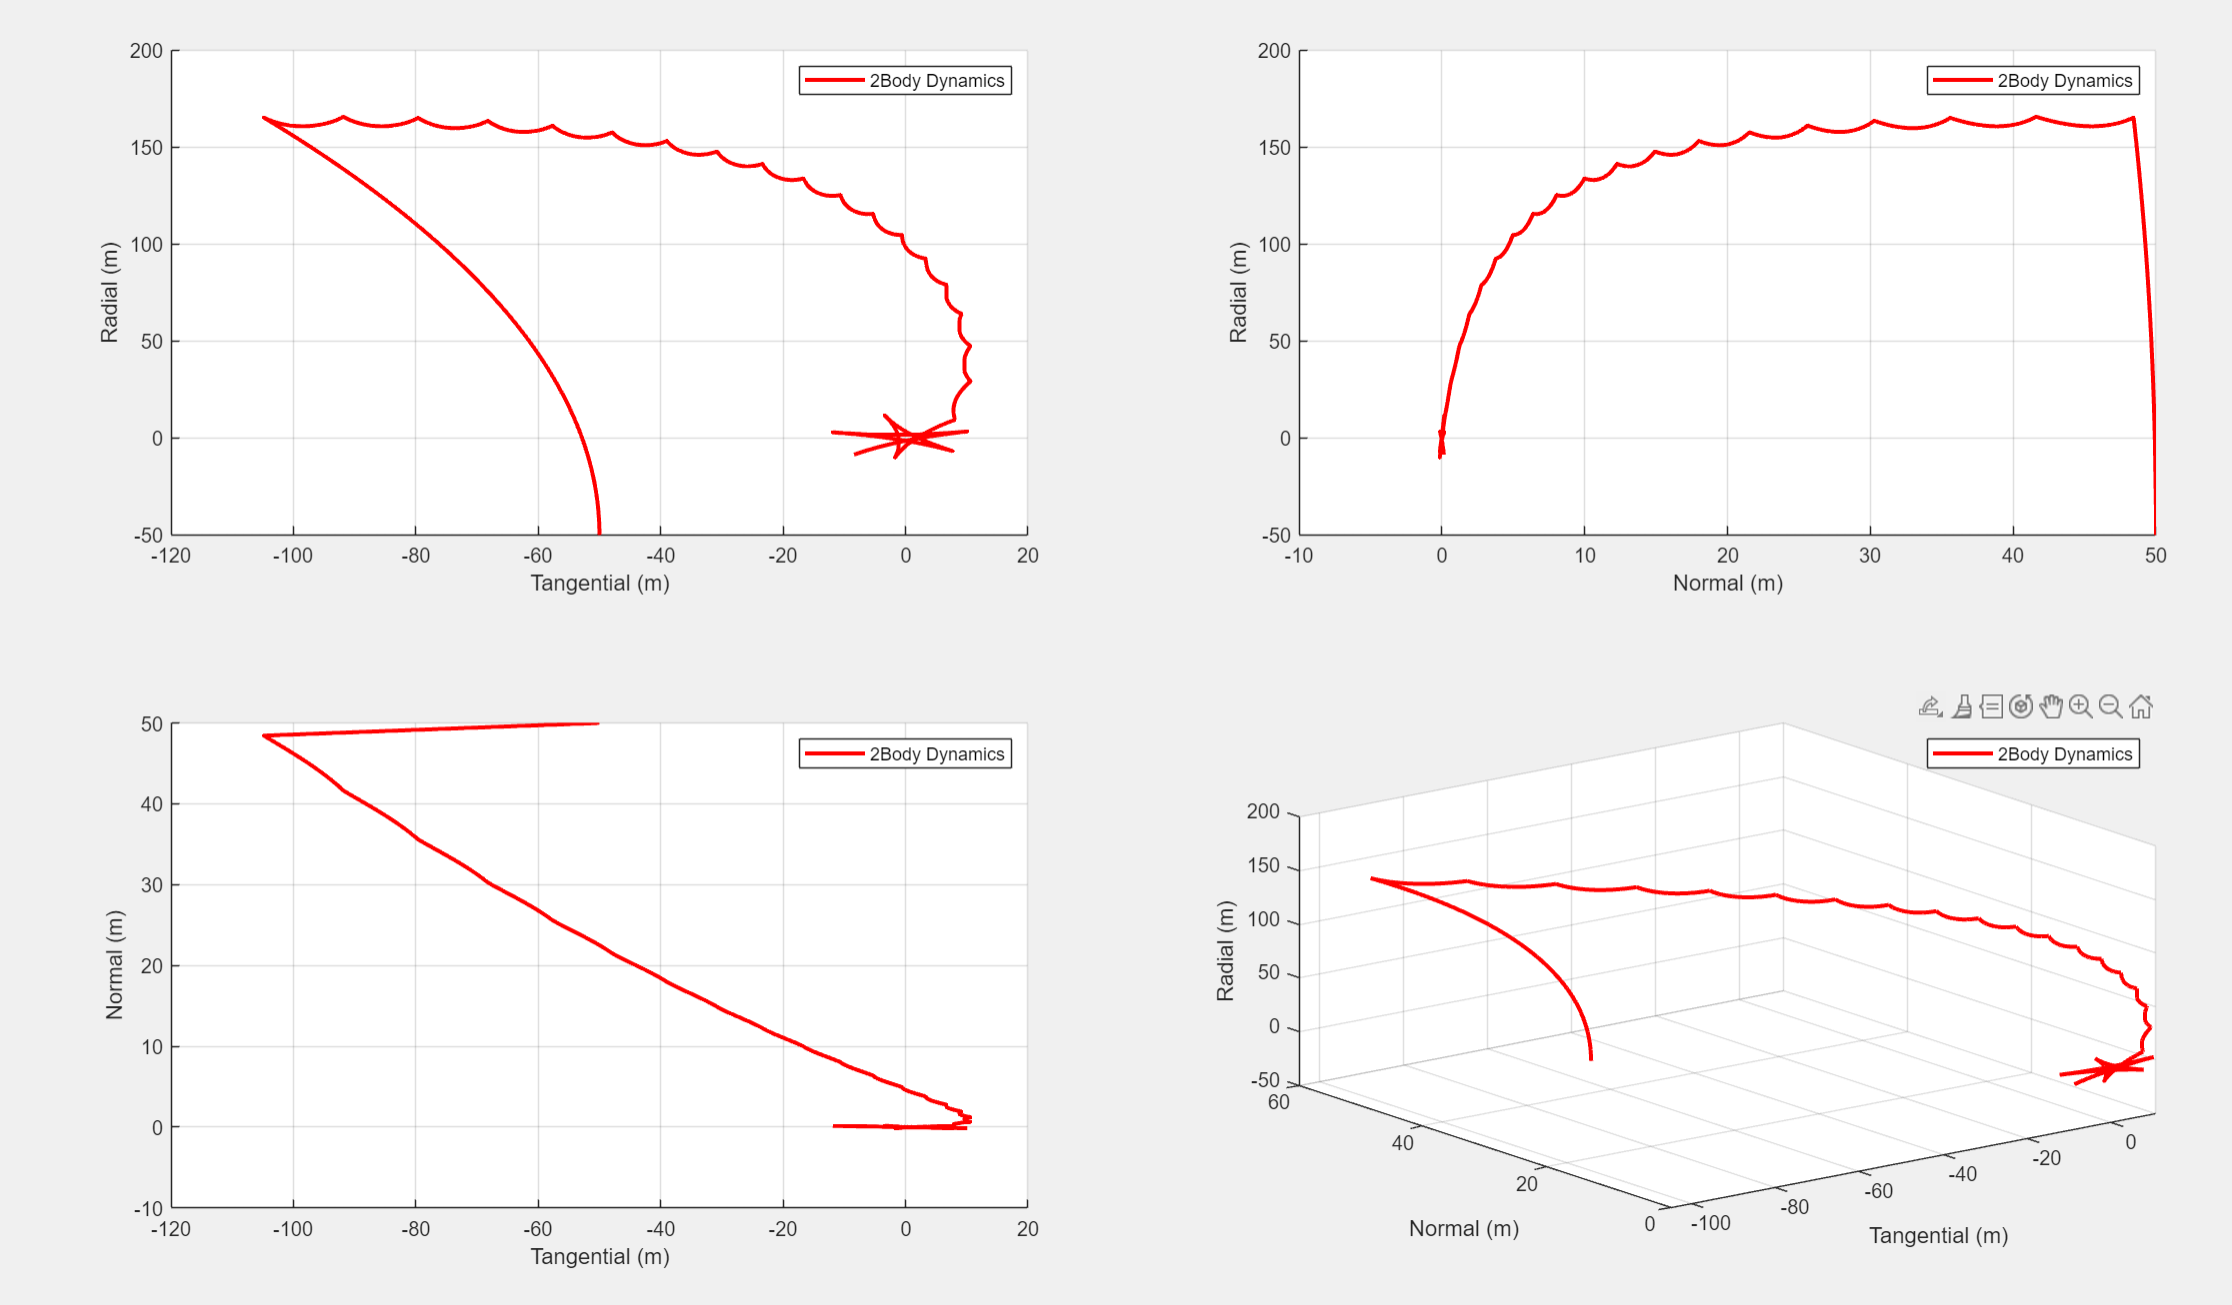
\includegraphics[width=0.7\textwidth]{PS5/Figures/position.png}
    \caption{RTN Trajectory}
    \label{fig:hcw_velocity}
\end{figure}

\begin{figure}[H]
    \centering
    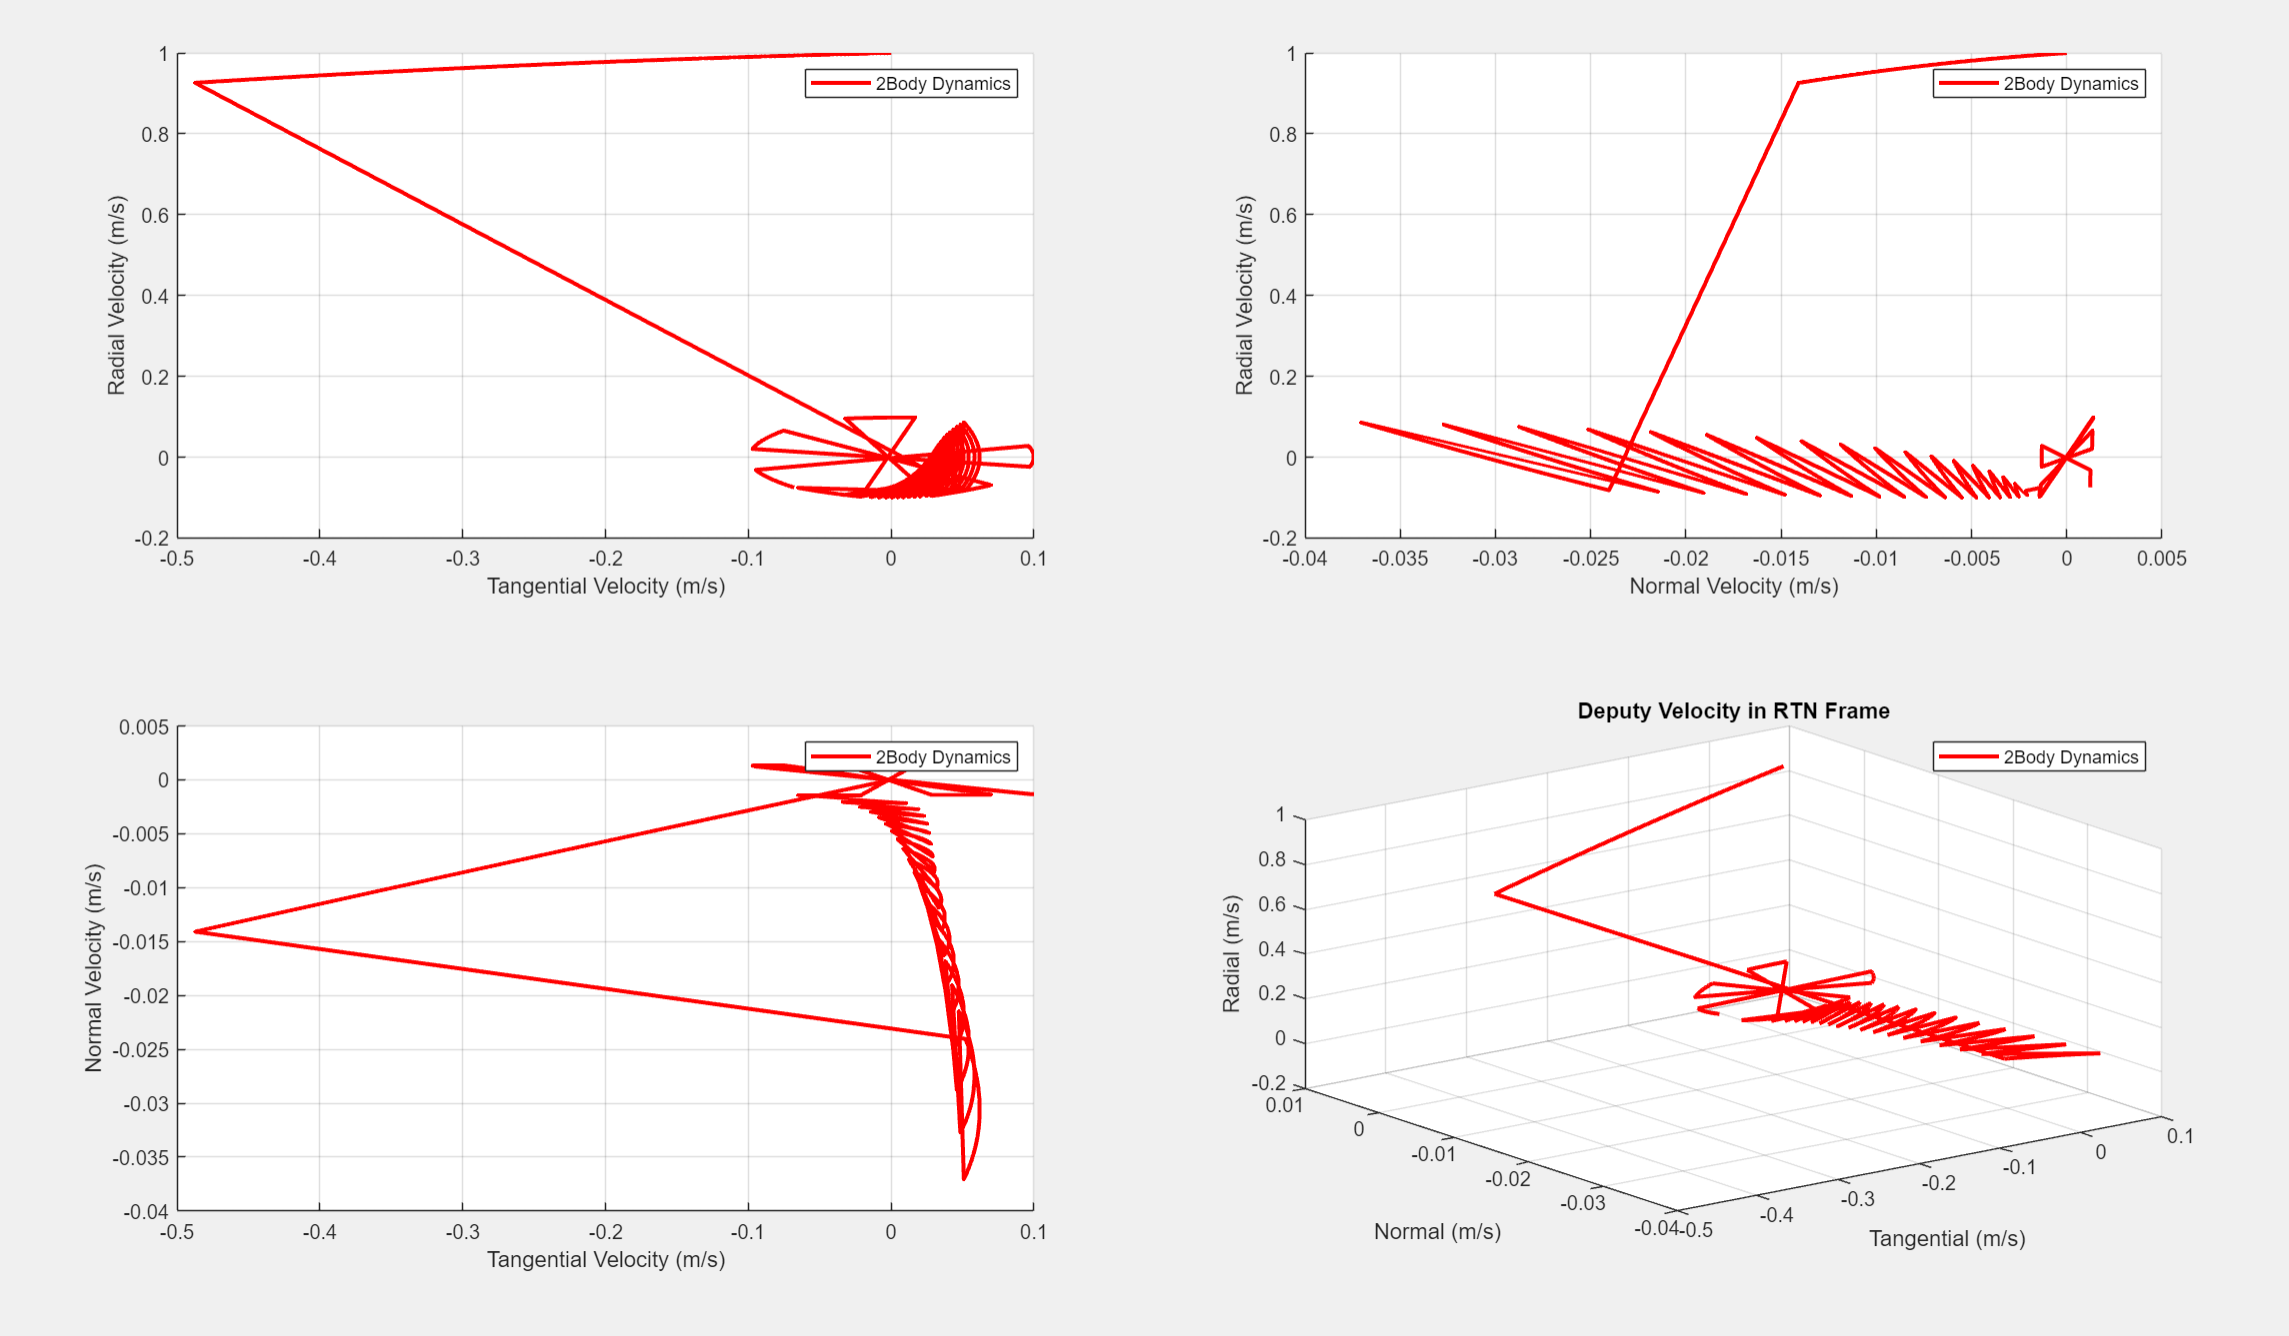
\includegraphics[width=0.7\textwidth]{PS5/Figures/velocity.png}
    \caption{RTN Velocity}
    \label{fig:hcw_velocity}
\end{figure}

\begin{figure}[H]
    \centering
    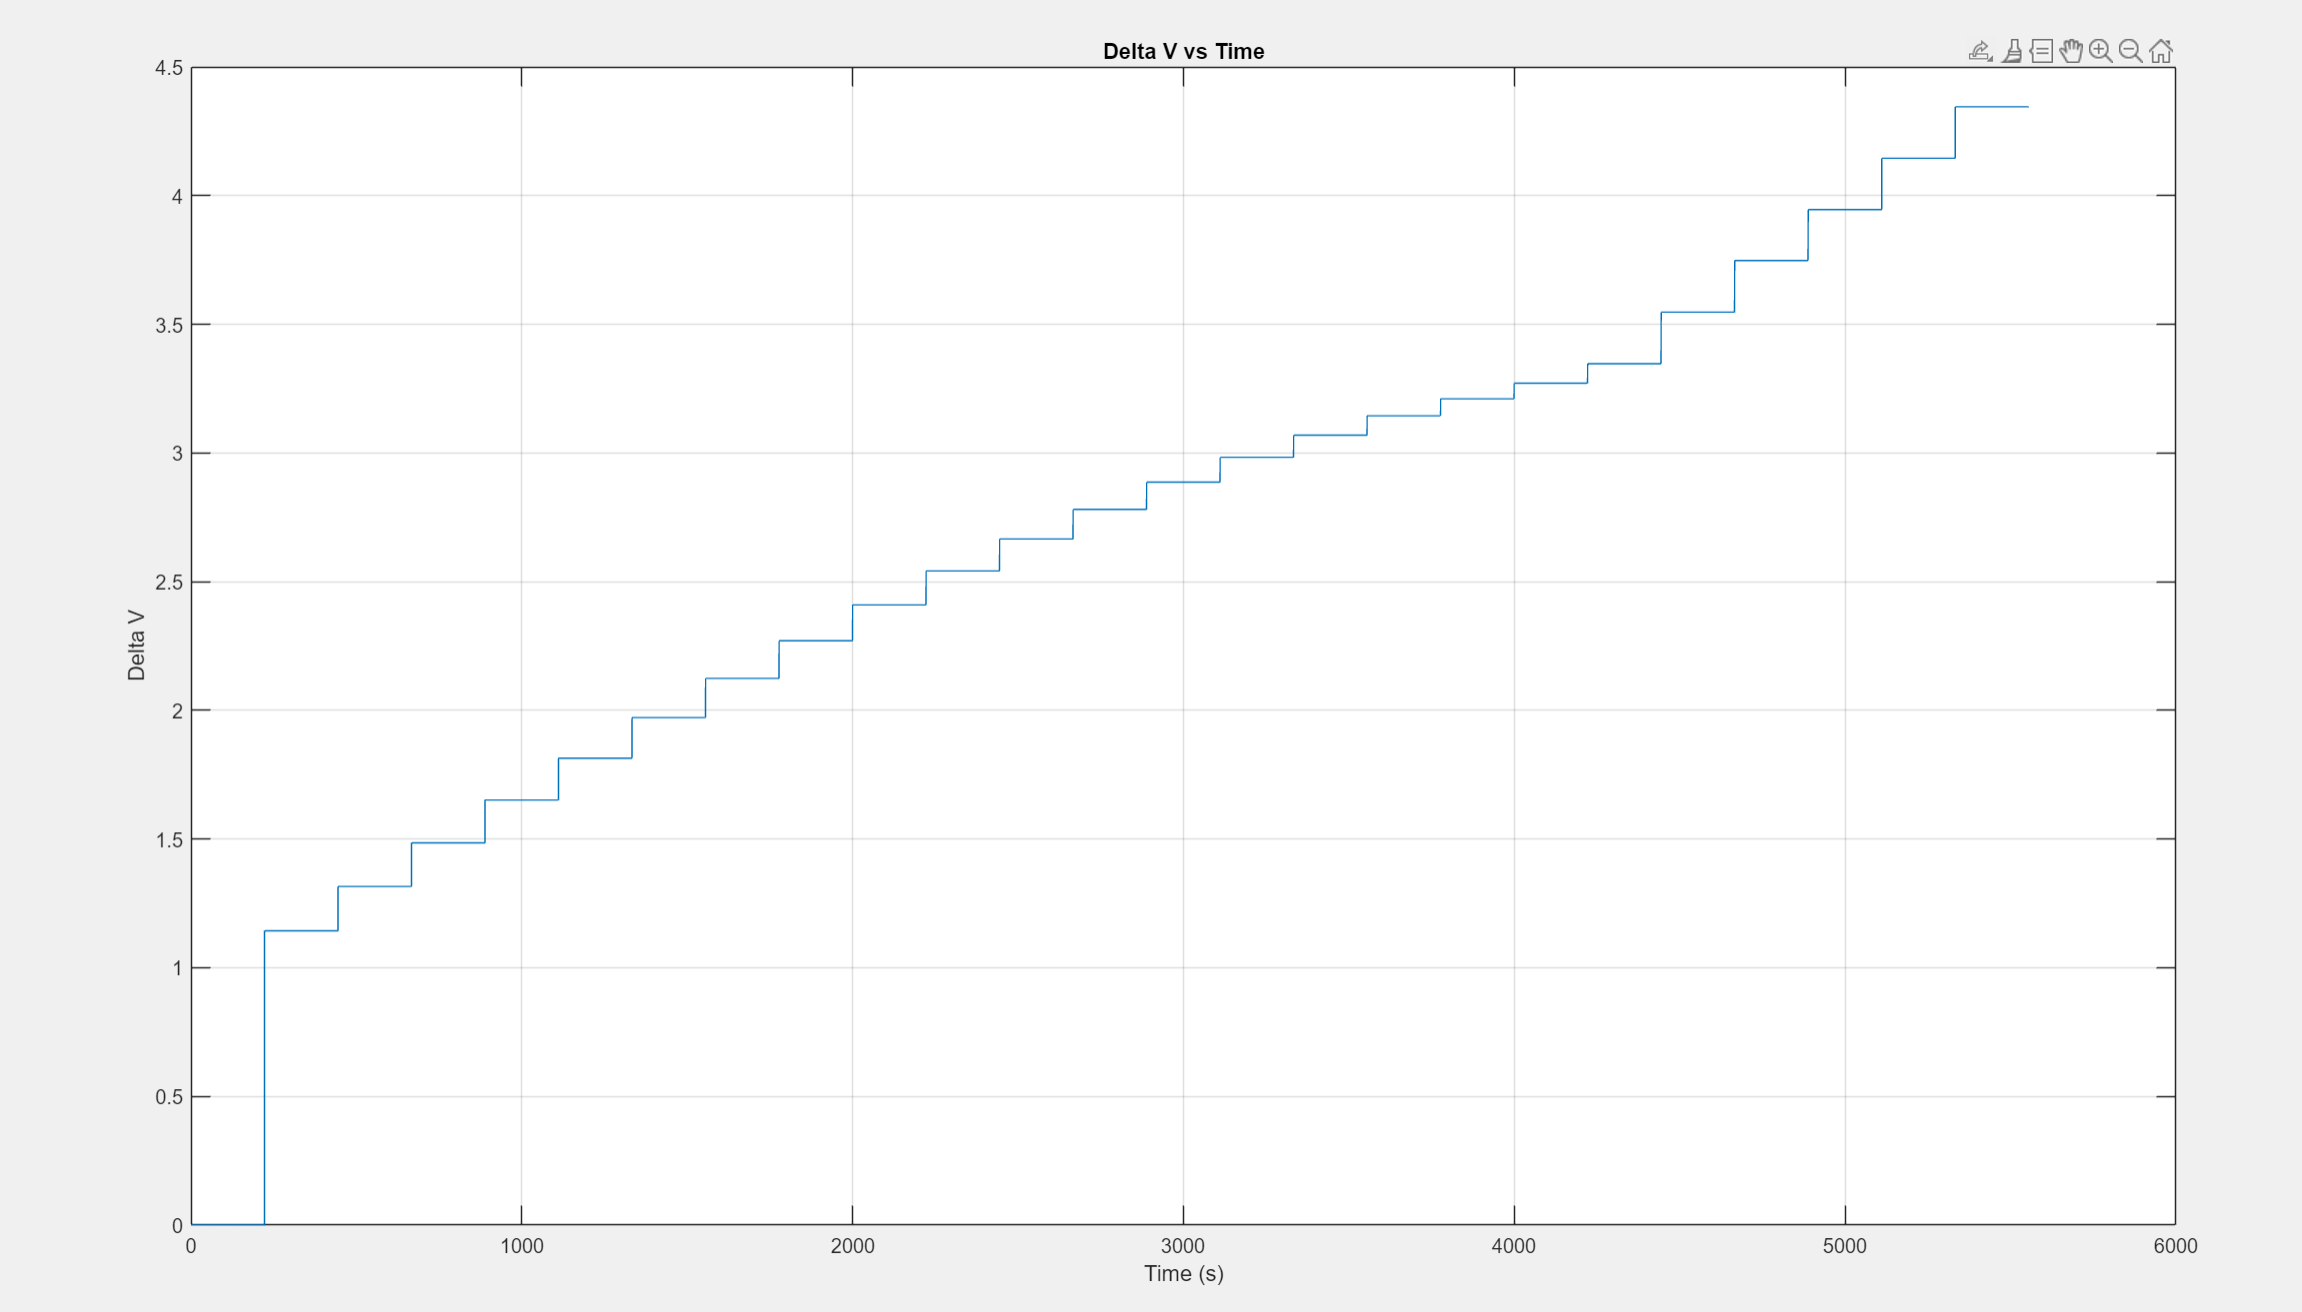
\includegraphics[width=0.7\textwidth]{PS5/Figures/dv.png}
    \caption{Dv usage over Time}
    \label{fig:hcw_velocity}
\end{figure}

As can be seen from the postion and velocity figures, the first burn is a significant one that cancels out most of the RTN velocity. From there, the algorithm proceeds in small steps to draw the spacecraft closer together, finally converging in a zone close to the chief.

The dv figure indicates a relatively low delta v of 4 m/s to converge a distance of 50m over the course of less than a third of an orbit.

